\chapter{Hierarhično razvrščanje besedil}
\label{ch:hierarhicno-razvrscanje-besedil}

Vrnimo se h Grimmovim pravljicam in ustvarimo naslednji delotok:

\begin{figure}[h]
    \centering
    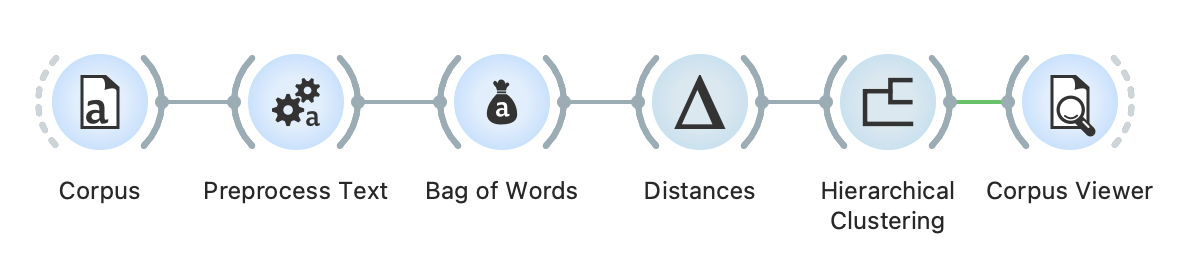
\includegraphics[width=\linewidth]{hc-workflow.png}%
    \caption{Enak delotok lahko preizkusite tudi na drugih podatkih, na primer na bookexcerpt.tab, ki vsebuje izvlečke knjig za odrasle in otroke.
    
    V tem primeru smo za razliko od prejšnje uporabili \textit{kosinusno razdaljo}. Pogostost besed iz vreče besed je predstavljena z vektorji, ki kažejo vsak v svojo smer glede na vsebino posameznega dokumenta. Kosinusna razdalja je kot med temi vektorji.}
    \label{fig:005-hc-workflow}
  \end{figure}

Gradnik \widget{Hierarchical Clustering} prikaže gruče v obliki dendrograma. Hierarchical Clustering povežite z gradnikom \widget{Corpus Viewer} in odprite oba gradnika. Izberite gručo v dendrogramu\marginnote{Beseda dendrogram je sestavljena iz grških besede dendro “drevo” in gramma “risba” in pomeni hierarhično vizualizacijo v obliki drevesa.} in v gradniku \widget{Corpus Viewer} poglejte, kateri dokumenti pripadajo izbrani skupini.

Raziščite različne gruče. Zakaj so nekatere magične pravljice (Tales of Magic) pomešane z živalskimi pravljicami (Animal Tales)? Kaj imajo skupnega?

\begin{figure*}[h]
    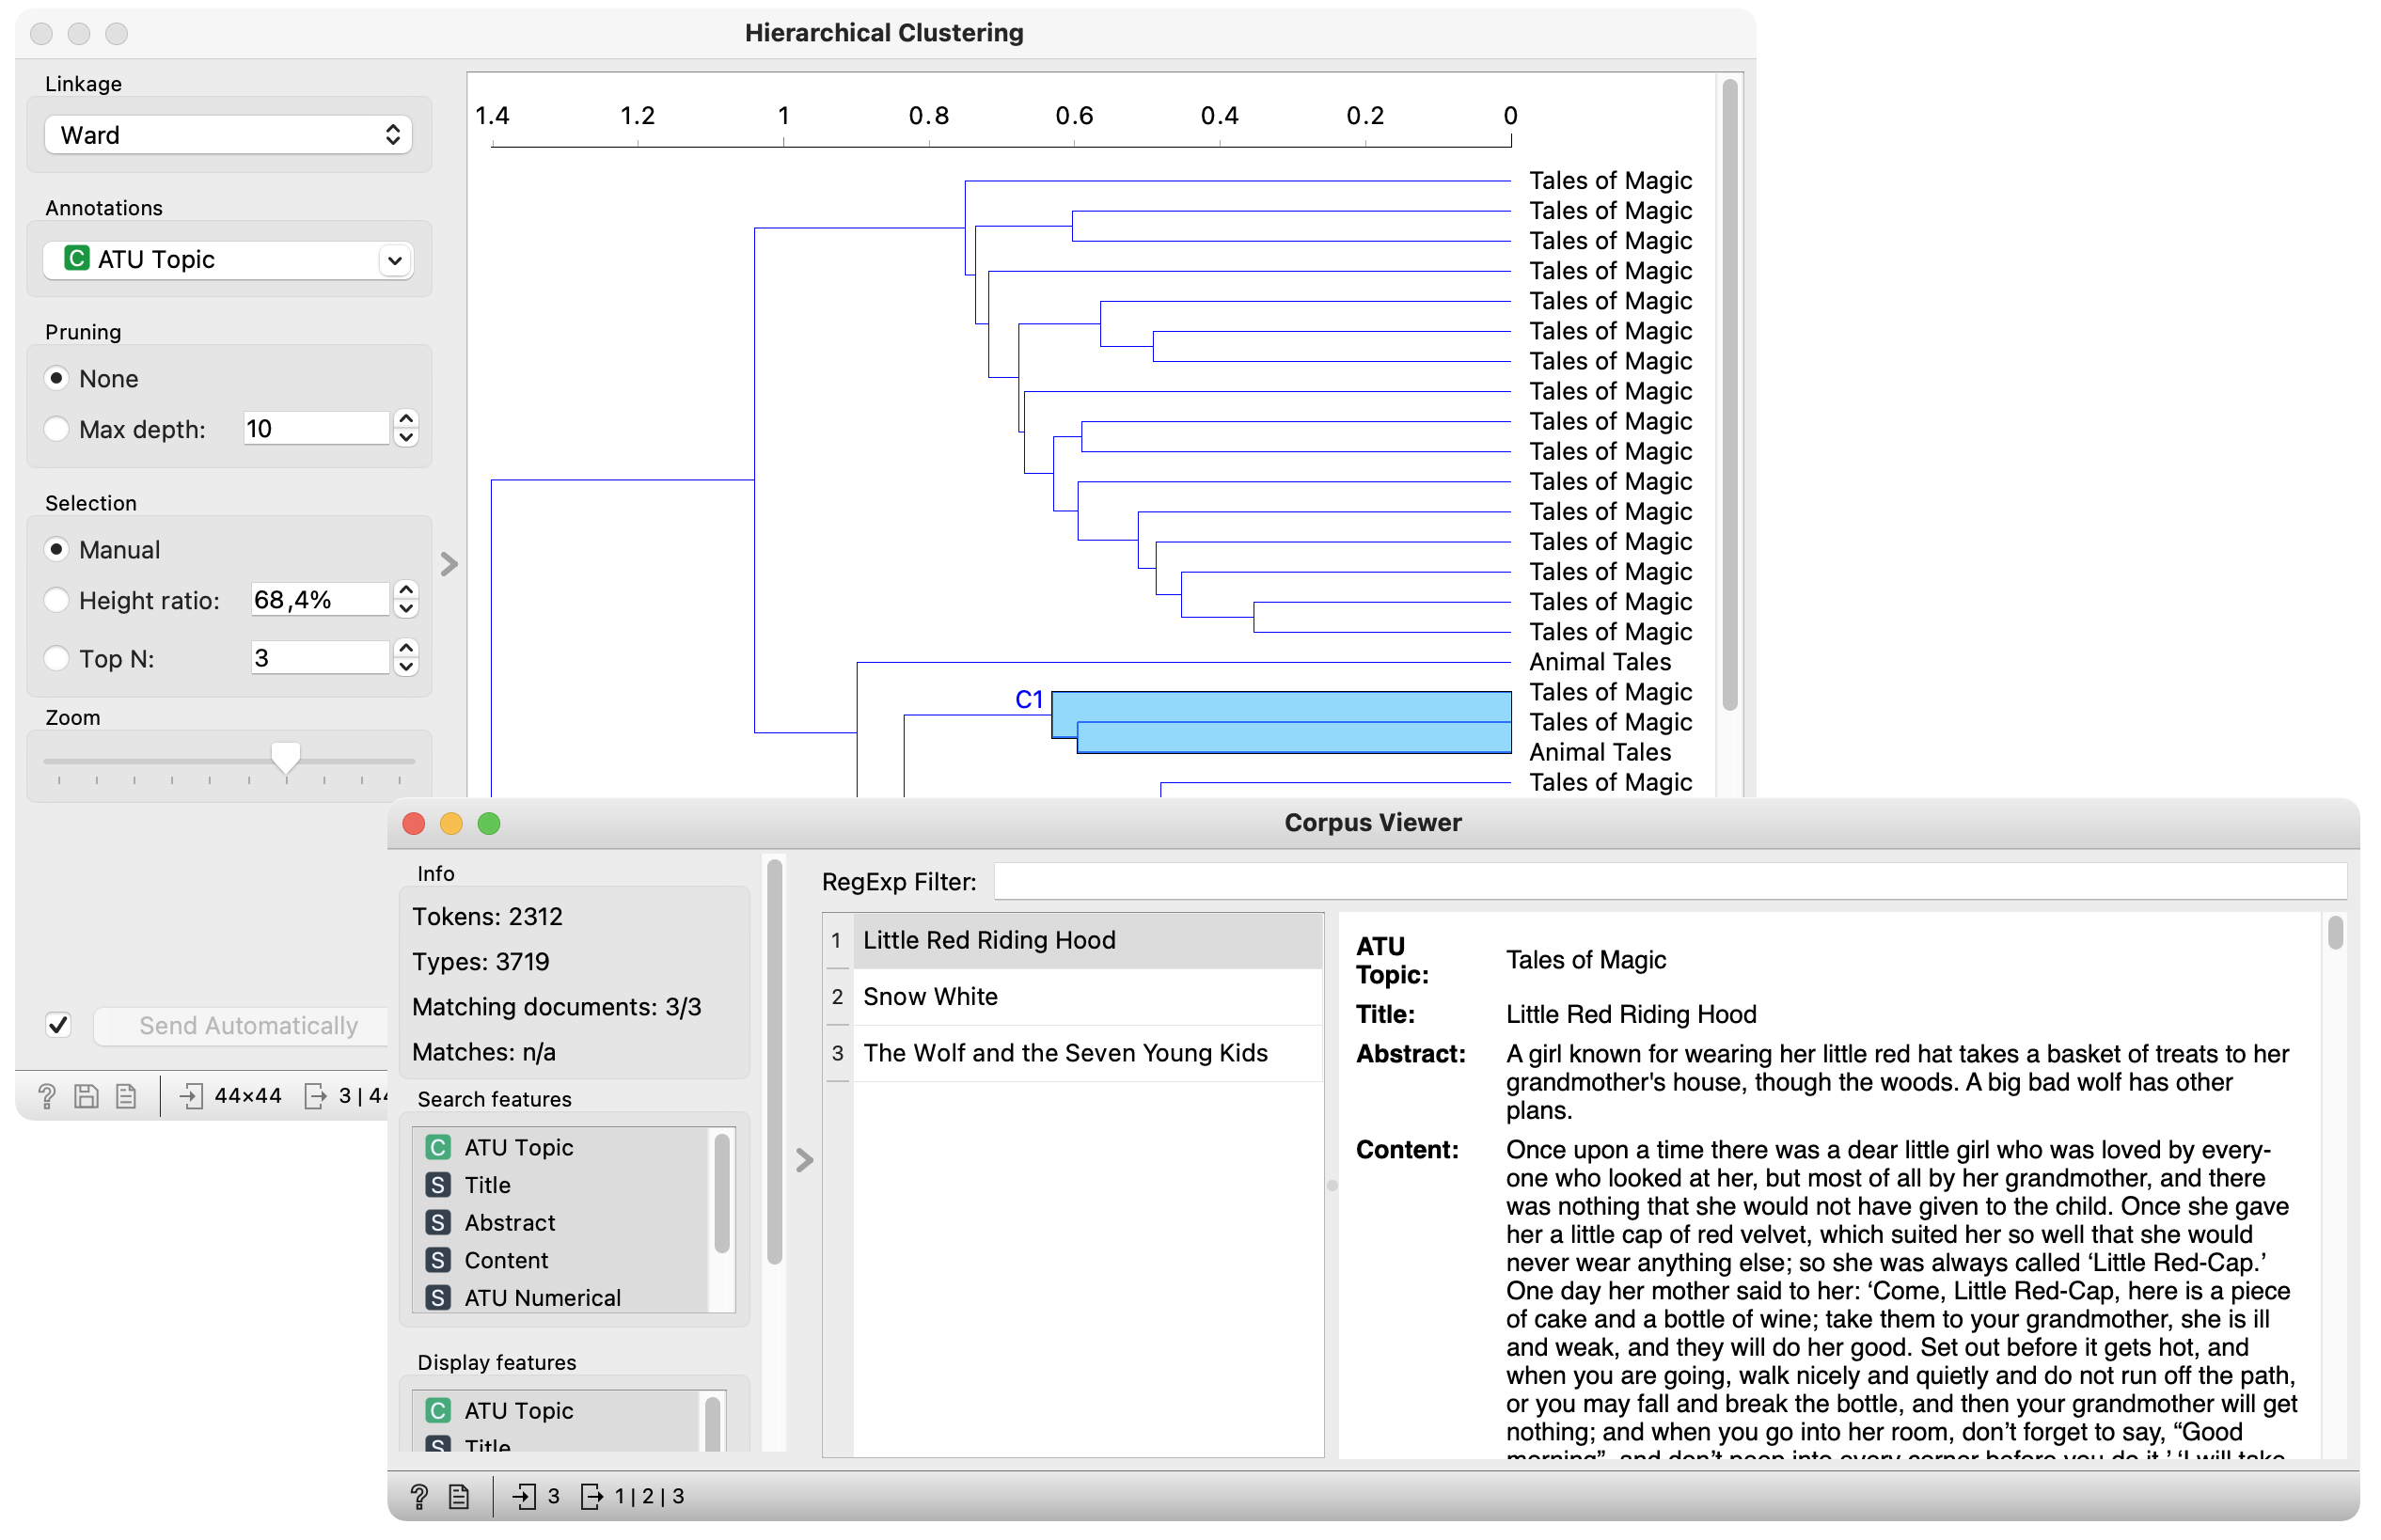
\includegraphics[width=\linewidth]{hc-one-cluster.png}%
    \caption{ }
    \label{fig:005-hc-one-cluster}
\end{figure*}

\newpage

Hierarhično razvrščanje zgradi hierarhijo dokumentov, mi pa se moramo odločiti, kje zamejimo podobnost znotraj skupine. Mejo podobnosti nastavimo tako, da na ravnilu zgoraj povlečemo črto desno ali levo in s tem zamejimo skupine.

Odločili smo se za pet skupin, saj po tem razdalja med skupinami kar precej naraste. Primerjajte pet skupin s štirimi, šestimi ali sedmimi. Gruče, ki jih odkrijemo, hkrati sovpadajo z oznako tipa Aarne-Thompson (ATU Topic).

\begin{figure*}[h]
    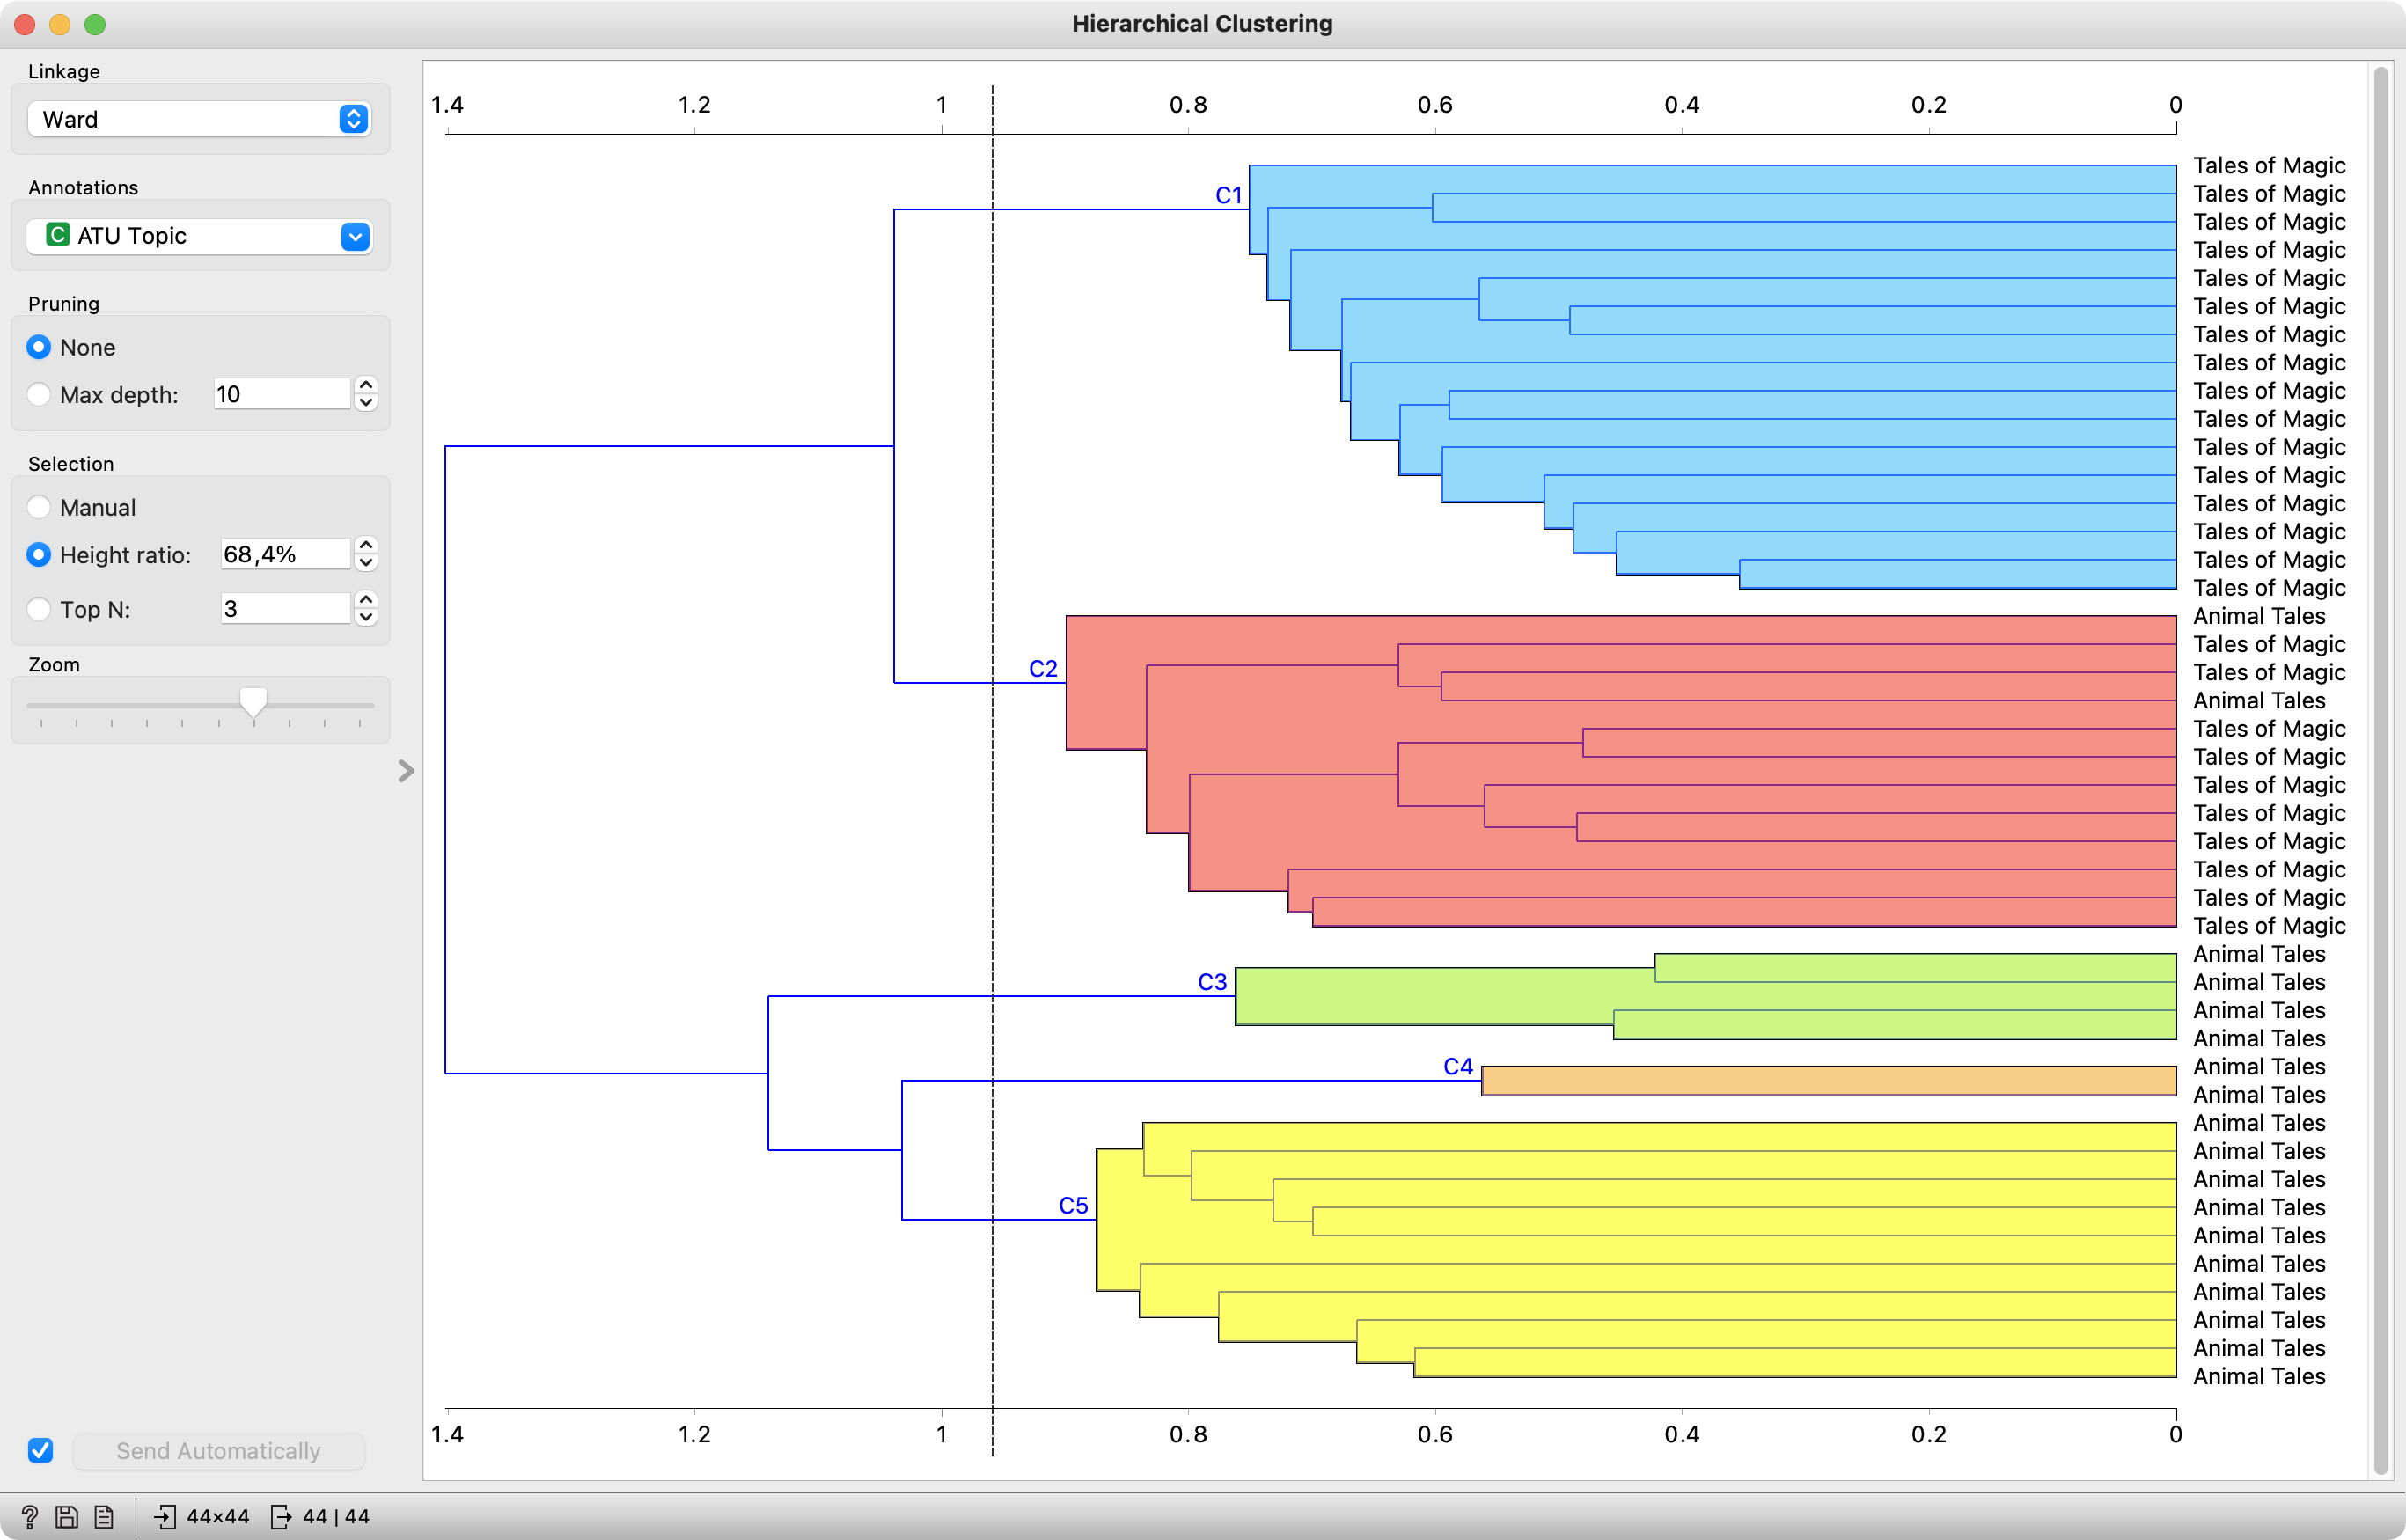
\includegraphics[width=\linewidth]{hc-clusters.png}%
    \caption{ }
    \label{fig:005-hc-clusters}
\end{figure*}

\newpage

Kako blizu pa so si v resnici živalske pravljice iz tretje in te iz četrte skupine? Ali ne bi bilo bolj zanimivo pogledati dokumente v ravnini, kjer bi se podobni dokumenti nahajali skupaj, različni pa narazen? Taka vizualizacija se imenuje večrazsežnostno lestvičenje oziroma \textit{Multidimensional Scaling (MDS)}.

\begin{figure*}[h]
    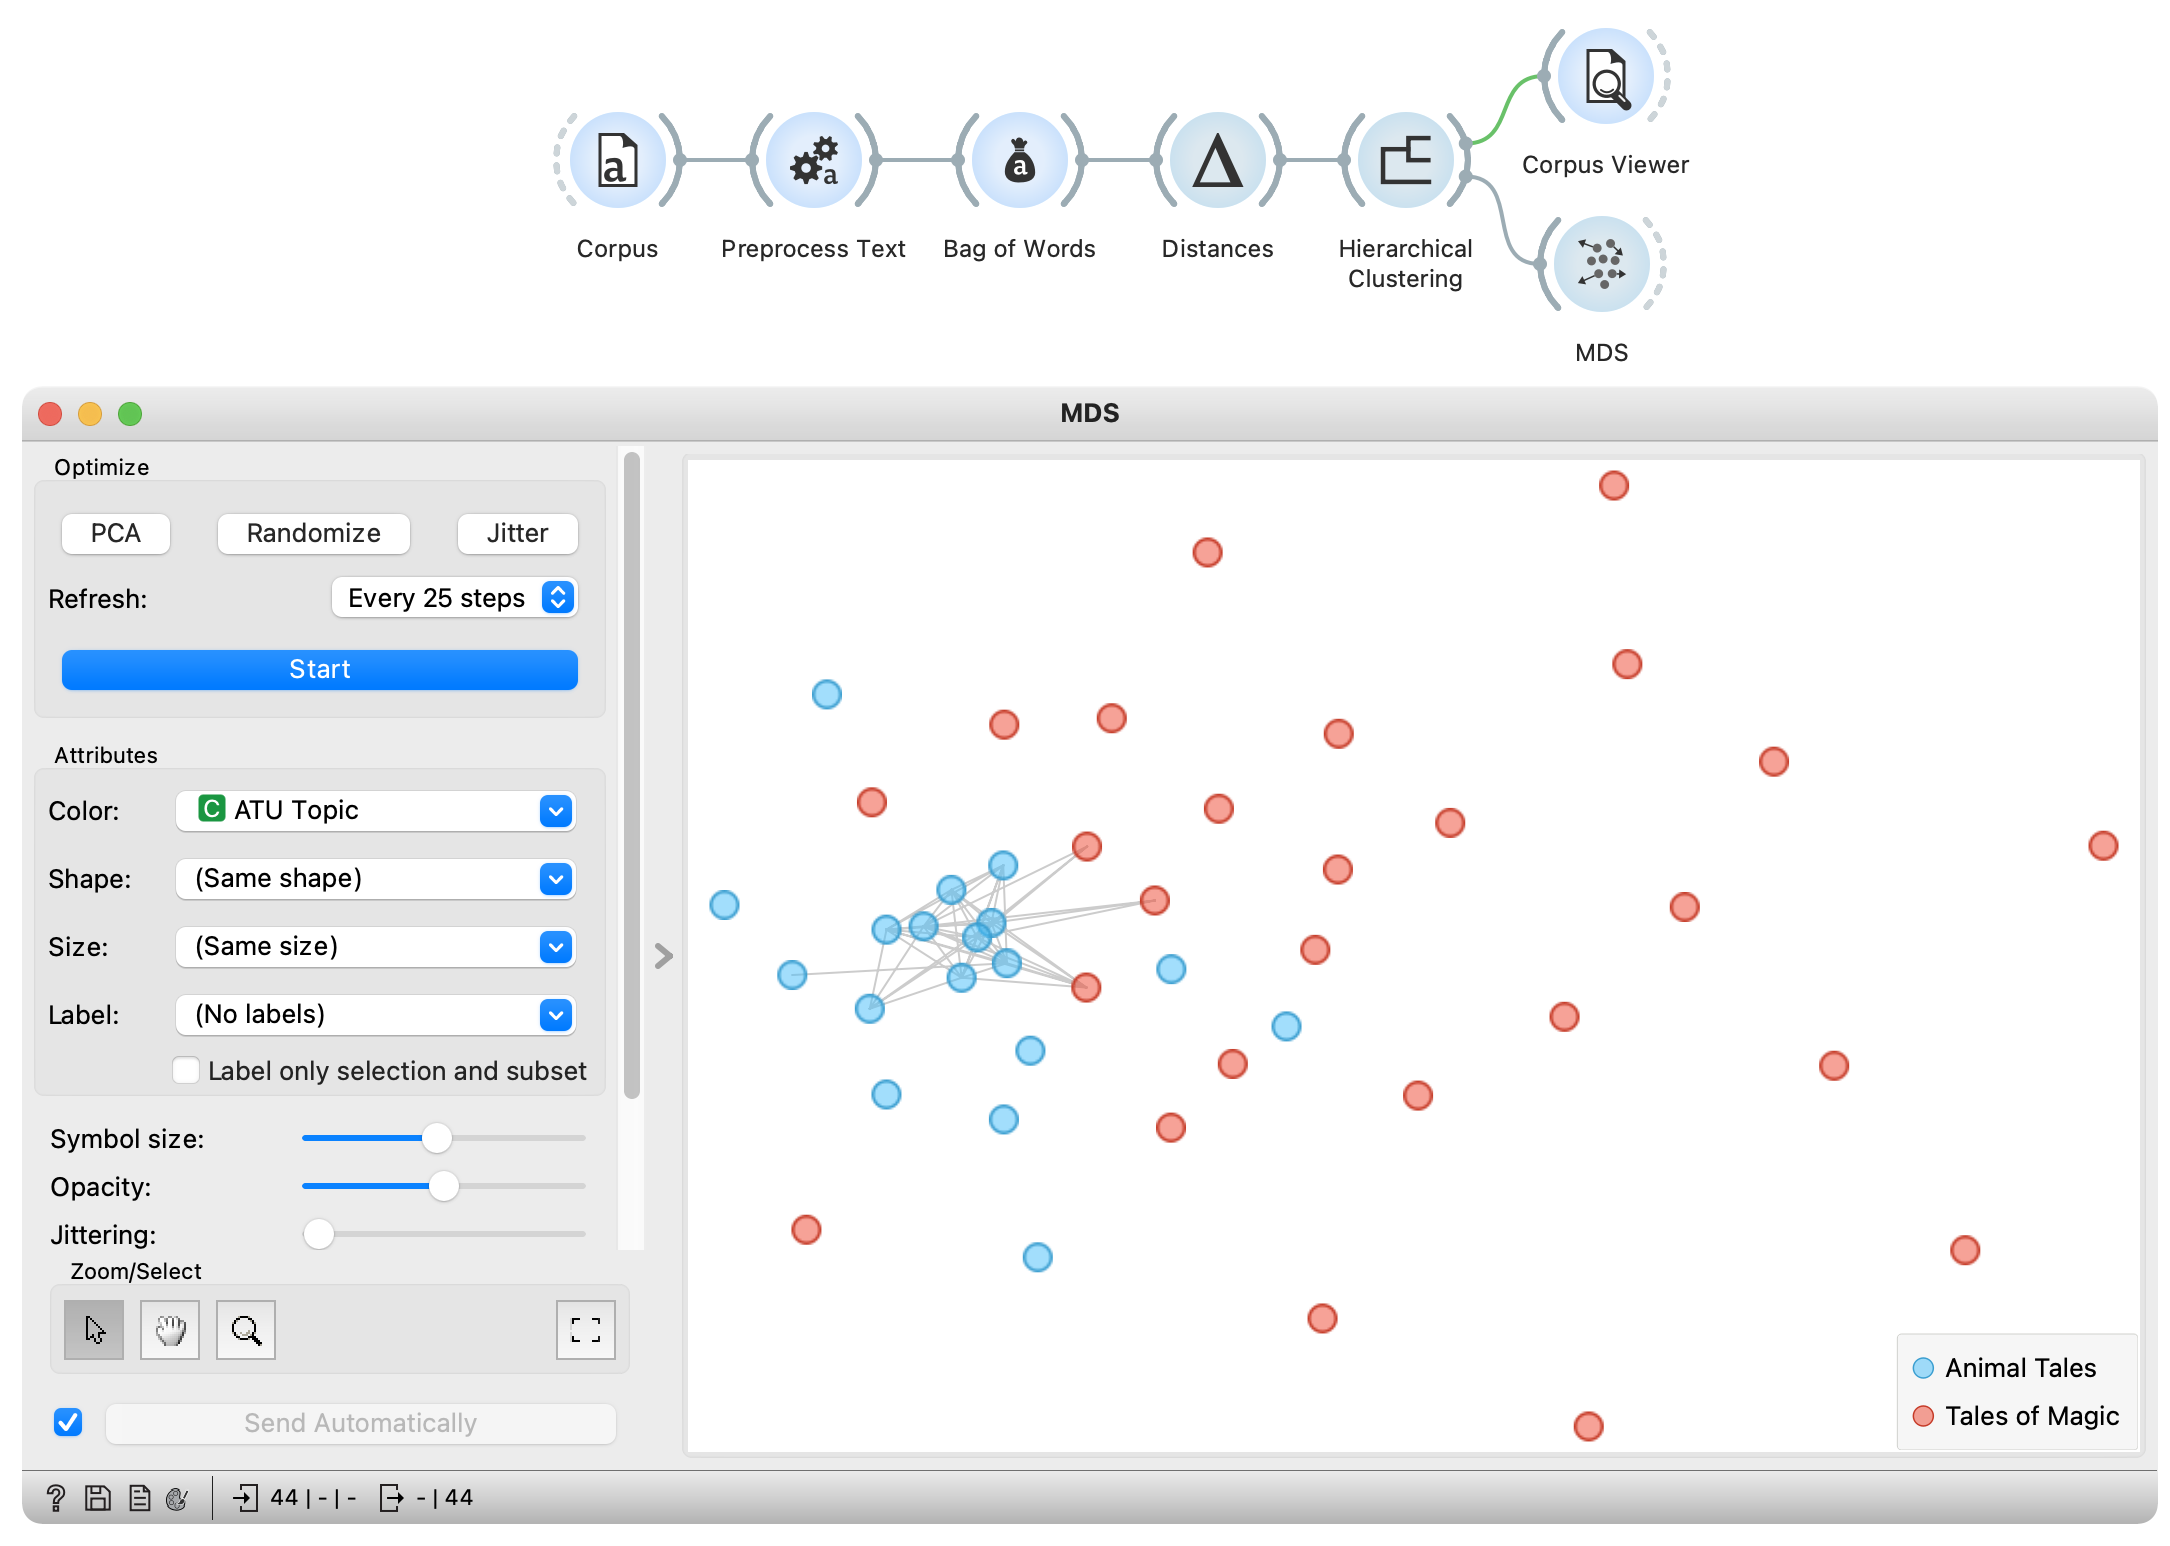
\includegraphics[width=\linewidth]{mds.png}%
    \caption{ }
    \label{fig:005-mds}
\end{figure*}

Magične pravljice tvorijo približno eno skupino, živalske pa drugo - tako kot smo pričakovali. Živalske pravljice so si med sabo bolj podobne kot magične (bolj so povezne). Raziščite podobne pravljice tako, da jih izberete v vizualizaciji in jih pogledate v gradniku Corpus Viewer.